\section{Taustayhteisöt}
\begin{figure}[htb]
	\begin{center}
		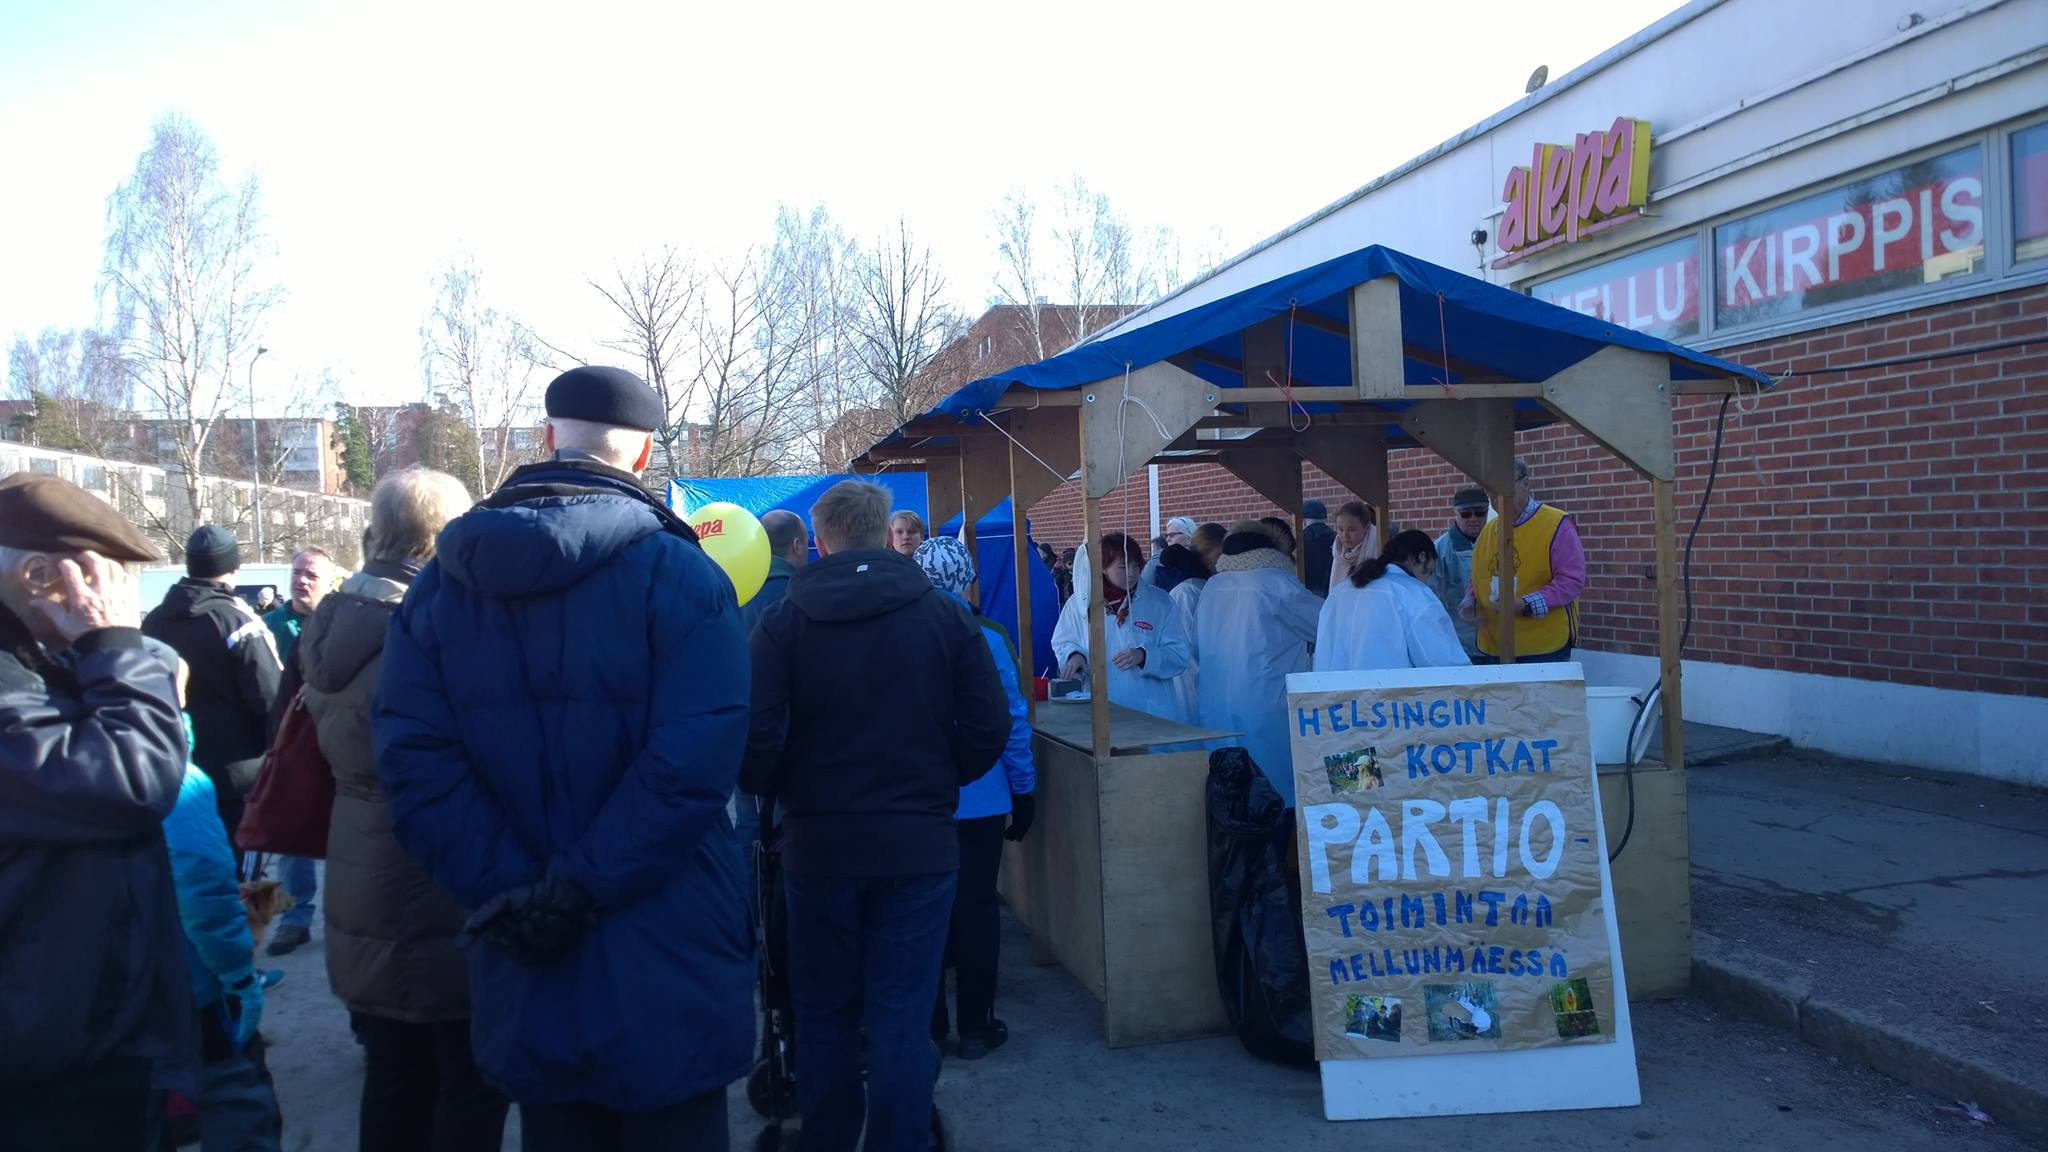
\includegraphics[height=7cm]{kuvat/lettukestit.jpg}
	\end{center}
	\captionsetup{labelformat=empty}
	\caption{\textbf{Vohvelimyyntiä Mellunmäen Lionsien kevätriehassa.}}
\end{figure}

Taustayhteisöinä ovat tuttuun tapaan toimineet Mikaelin seurakunta, Mellunmäen Lions Club ja Partiolippukunta Helsingin Kotkat ry:n Venhempainyhdistys ry. Jokaiseen taustayhteisöön on oltu aktiivisesti yhteydessä ja heidän kanssaan on järjestetty tapahtumia.\\
\\Lippukunta oli useaan otteeseen mukana auttamassa Mikaelin seurakunnan tapahtumissa keräämällä mm. kolehtia ja nostamalla lipun itsenäisyyspäivänä. Yhteistyö Mellunmäen Lions Clubin kanssa rajoittui lähinnä avustamiseen kevätriehassa ja itsenäisyyspäivän lipunnostoon Mellunmäen ostoskeskuksen edustalla, mutta yhteydenpito oli silti erittäin aktiivista ja molemmin puolin vallitsi herrasmiessopimus siitä, että apua annetaan tarvittaessa puolin ja toisin.\\
\\Vanhempainyhdistys oli tuttuun tapaansa todella tärkeässä asemassa lippukunnan toiminnan kannalta, sen kanssa järjestettiin Kyöpelin talkoot sekä keväinen iltapäiväretki jätelaitokselle. 

